\documentclass{article}
\newcommand{\BEAS}{\begin{eqnarray*}}
\newcommand{\EEAS}{\end{eqnarray*}}
\newcommand{\BEQ}{\begin{equation}}
\newcommand{\EEQ}{\end{equation}}
\newcommand{\BIT}{\begin{itemize}}
\newcommand{\EIT}{\end{itemize}}

\newcommand{\eg}{{\it e.g.\ }}
\newcommand{\ie}{{\it i.e.\ }}

\newcommand{\ones}{\mathbf 1}
\newcommand{\zeros}{\mathbf 0}
\newcommand{\reals}{{\mbox{\bf R}}}
\newcommand{\integers}{{\mbox{\bf Z}}}
\newcommand{\symm}{{\mbox{\bf S}}}  % symmetric matrices

\newcommand{\nullspace}{{\mathcal N}}
\newcommand{\range}{{\mathcal R}}
\newcommand{\Rank}{\mathop{\bf Rank}}
\newcommand{\Tr}{\mathop{\bf Tr}}

\newcommand{\sign}[1]{\mathop{\textrm{sgn}}(#1)}
\newcommand{\lambdamax}{{\lambda_{\rm max}}}
\newcommand{\lambdamin}{\lambda_{\rm min}}

\newcommand{\EE}{\mathop{\textrm{E}}}
\newcommand{\Cov}{\mathop{\textrm{Cov}}}
\newcommand{\Prob}{\mathop{\bf Prob}}
\newcommand{\Co}{{\mathop {\bf Co}}} % convex hull
\newcommand{\dist}{\mathop{\bf dist{}}}
\newcommand{\argmin}{\mathop{\rm argmin}}
\newcommand{\argmax}{\mathop{\rm argmax}}
\newcommand{\epi}{\mathop{\bf epi}} % epigraph
\newcommand{\Vol}{\mathop{\bf vol}}
\newcommand{\dom}{\mathop{\bf dom}} % domain
\newcommand{\intr}{\mathop{\bf int}}


\newcommand{\nrm}[1]{\left\lVert#1\right\rVert}
\newcommand{\nrmo}[1]{\left\lVert#1\right\rVert_1}
\newcommand{\nrmt}[1]{\left\lVert#1\right\rVert_2}
\newcommand{\nrmnn}[1]{\left\lVert#1\right\rVert_{*}}
\newcommand{\nrmf}[1]{\left\lVert#1\right\rVert_F}

\newcommand{\myexp}[1]{\mathop{\rm exp}\left\{#1\right\}}
\newcommand{\mylog}[1]{\mathop{\rm log}\left\{#1\right\}}
\newcommand{\questions}{\begin{frame}Questions?\end{frame}}
\newcommand{\LL}{\textrm{LL}}
\newcommand{\KL}{\textrm{KL}}
\newcommand{\HH}{\textrm{H}}
\newcommand{\GG}{\textrm{G}}

\newcommand{\Bound}{\textrm{B}}
\newcommand{\bb}{\mathbf{b}}
\newcommand{\aaa}{\mathbf{a}}
\newcommand{\BB}{\mathbf{B}}
\newcommand{\AAA}{\mathbf{A}}
\newcommand{\CC}{\mathbf{C}}
\newcommand{\cc}{\mathbf{c}}
\newcommand{\mm}{\mathbf{m}}
\newcommand{\MM}{\mathbf{M}}
\newcommand{\nn}{\mathrm{\bf neighbors}}
\newcommand{\pa}[1]{{\textrm{\bf pa}}\left(#1\right)}
\newcommand{\pre}[2]{\mathop{\textrm{\bf pnp}}_{#1}\left(#2\right)}
\newcommand{\logsum}{\textrm{logsum}}

\newcommand{\tth}{{\textrm{th}}}
\newcommand{\xx}{\mathbf{x}}
\newcommand{\mmu}{\mathbf{\mu}}
\newcommand{\yy}{\mathbf{y}}
\newcommand{\zz}{\mathbf{z}}
\newcommand{\dd}{\mathbf{d}}
\newcommand{\new}{\textrm{new}}
\newcommand{\old}{\textrm{old}}
\newcommand{\fpr}{\textrm{FPR}}
\newcommand{\tpr}{\textrm{TPR}}
\newcommand{\auc}{\textrm{AUC}}
\newcommand{\yyi}{\yy_i}
\newcommand{\xxi}{\xx_i}
\newcommand{\vvec}[2]{\left[ \begin{array}{c} \mathbf{#1}\\ \mathbf{#2} \end{array}\right]}
\newcommand{\mmat}[4]{\left[ \begin{array}{cc} \mathbf{#1}&\mathbf{#2}\\ \mathbf{#3}&\mathbf{#4} \end{array}\right]}
\newcommand{\xyvec}{\left[ \begin{array}{c} \xx\\\yy \end{array} \right]}
\newcommand{\xyvecc}{\left[ \begin{array}{c} x^1\\y^1 \end{array} \right]}
\newcommand{\eye}{   \left[ \begin{array}{cc} 1 & 0 \\ 0 & 1 \end{array}\right]}
\newcommand{\bket}[2]{\left\langle#1,#2\right\rangle}
\newcommand{\bbket}[2]{\left\llangle#1,#2\right\rrangle}
\newcommand{\redq}{\textcolor{red}{q}}
\newcommand{\blup}{\textcolor{blue}{p}}
\newcommand{\BIEA}{\begin{IEEEeqnarray*}}
\newcommand{\EIEA}{\end{IEEEeqnarray*}}
\newcommand{\BIEAN}{\begin{IEEEeqnarray}}
\newcommand{\EIEAN}{\end{IEEEeqnarray}}
\newcommand{\pmin}{\mathop{\textrm{minimize}}}
\newcommand{\psubjto}{\textrm{subject to}}
\newcommand{\WW}{\mathbf{W}}
\newcommand{\ww}{\mathbf{w}}
\newcommand{\YY}{\mathbf{Y}}
\newcommand{\XX}{\mathbf{X}}
\newcommand{\UU}{\mathbf{U}}
\newcommand{\uu}{\mathbf{u}}
\newcommand{\VV}{\mathbf{V}}
\newcommand{\vv}{\mathbf{v}}
\newcommand{\PP}{\mathbf{P}}
\newcommand{\pp}{\mathbf{p}}
\newcommand{\rr}{\mathbf{r}}
\newcommand{\RR}{\mathbf{R}}
\newcommand{\ee}{\mathbf{e}}
\newcommand{\II}{\mathbf{I}}
\newcommand{\DD}{\mathbf{D}}

\newcommand{\aalpha}{{\boldsymbol\alpha}}
\newcommand{\llambda}{{\boldsymbol\lambda}}
\newcommand{\ddelta}{{\boldsymbol\delta}}
\newcommand{\otherwise}{\textrm{otherwise}}
\newcommand{\answer}{\fbox{\tt answer} }
\newcommand{\abs}[1]{\left| #1 \right|}

\newcounter{problemCtr}
\newcommand{\newproblem}[1]{\hrule\paragraph{Problem \theproblemCtr (#1)}\stepcounter{problemCtr}}


\newcounter{HW}

\usepackage{amsthm}
\usepackage{graphicx}
\usepackage{natbib}
\usepackage{algorithm}
\usepackage{algorithmic}
\usepackage{amsmath}
\usepackage{hyperref}
\usepackage{tikz}


\newtheorem{remark}{Remark}
\newtheorem{lemma}{Lemma}
\newtheorem{definition}{Definition}
\newtheorem{proposition}{Proposition}
\newtheorem{assumption}{Assumption}
\newtheorem{corollary}{Corollary}
\newtheorem{theorem}{Theorem}


\setcounter{HW}{1}
\begin{document}

\author{Ravikiran Janardhana}
\title{COMP  790-124, HW\theHW}
\maketitle



\newproblem{0.01pt} Open \texttt{hw\theHW.tex}, replace ``Wile E. Coyote'' with your name. Run
\texttt{pdflatex hw\theHW.tex}, look at hw\theHW.pdf, and confirm that your name is in the right place.


\newproblem{1pt}
\begin{enumerate}
\item Plot the sigmoid function in MATLAB using script
\begin{verbatim}
z = [-5:0.1:5];
fz = 1./(1 + exp(-z));
plot(z,fz,'LineWidth',3);
xlabel('z');ylabel('f(z)'); % we always label axes, yes we do!
hwplotprep
print -dpdf sigmoid.pdf
\end{verbatim}
Find the resulting figure in file {\tt sigmoid.pdf}.
b) In hw\theHW.tex, find the segment of the file that sets up the first figure -- it starts with {\tt \textbackslash begin\{figure\}} and ends with  {\tt \textbackslash end\{figure\}}.
\item Inside this segment  replace {\tt emptiness.pdf} with {\tt sigmoid.pdf}.
\item Change the text under {\tt \textbackslash caption} -- right now it says ``This is emptiness, it earns no points.'' -- to say what the figure is about.
\item Remake hw\theHW.pdf by running in shell/command prompt

     \texttt{pdflatex hw\theHW.tex}

and check that your plot and caption are now in.
\end{enumerate}


\begin{figure}[H]
\begin{center}
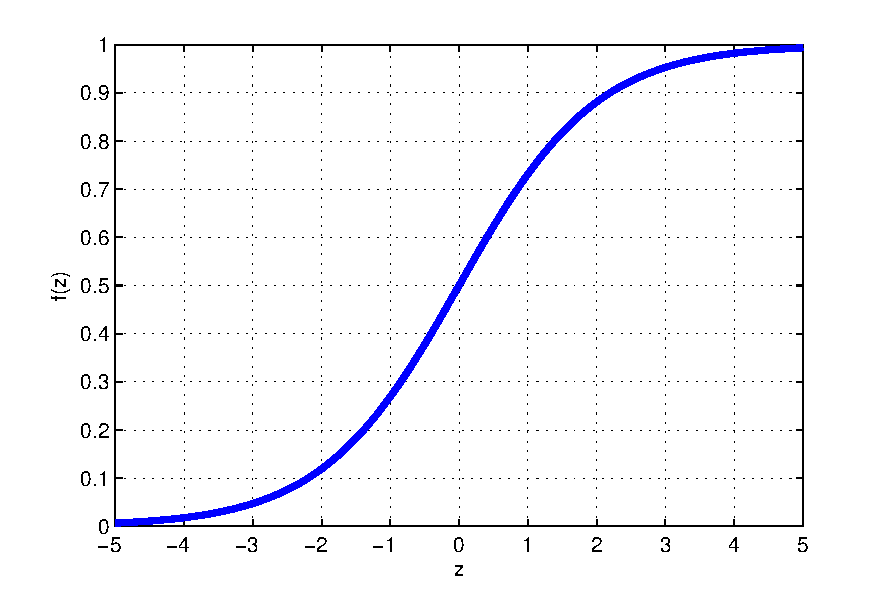
\includegraphics[scale=0.5]{sigmoid.pdf}
\caption{Plot of Sigmoid Function}
\end{center}
\end{figure}

\hrule

\newproblem{1pt}
Fill in the first derivative and second derivative of sigmoid function in the hw\theHW.tex.

Sigmoid funcion
\[
f(z) = \frac{1}{1+e^{-z}} 
\]

The first derivative
\[
\frac{d f(z)}{dz} = f(z) * (1 - f(z)) = \frac{1}{e^{z}(1+e^{-z})^{2}}
\]

The second derivative
\[
\frac{d^{2} f(z)}{d{z}^{2}} = \frac{d f(z)}{dz} * (1 - 2f(z)) = \frac{1 - e^{z}}{e^{2z}(1+e^{-z})^{3}}
\]


\newproblem{1pt}
Write a MATLAB function that implements computation  of the first derivative of $f$ at a particular point. You just did the math for this.
\begin{verbatim}
function d = dsigmoid(z)
    % This function computes first derivative of sigmoid function at z
    d = 1 ./ (exp(z) .* (1+exp(-z)).^2);
end
\end{verbatim}

Crate a file {\tt dsigmoid.m} that {\em correctly} computes the first derivative.

\newproblem{1pt}

We will use your function {\tt dsigmoid.m} to plot the first derivative.
\begin{verbatim}
zs = [-5:0.01:5];
for i = 1:length(zs)
    ds(i) = dsigmoid(zs(i));
end
plot(zs,ds,'LineWidth',3);
xlabel('z');ylabel('df(z)');
hwplotprep
print -dpdf dsigmoid.pdf
\end{verbatim}

Find the resulting plot in file {\tt dsigmoid.pdf}. In hw\theHW.tex replace {\tt emptiness.pdf} with {\tt dsigmoid.pdf} . Change the
caption in the figure to say what the figure is about. Remake hw\theHW.pdf and check that your plot has made it in.
\begin{figure}[H]
\begin{center}
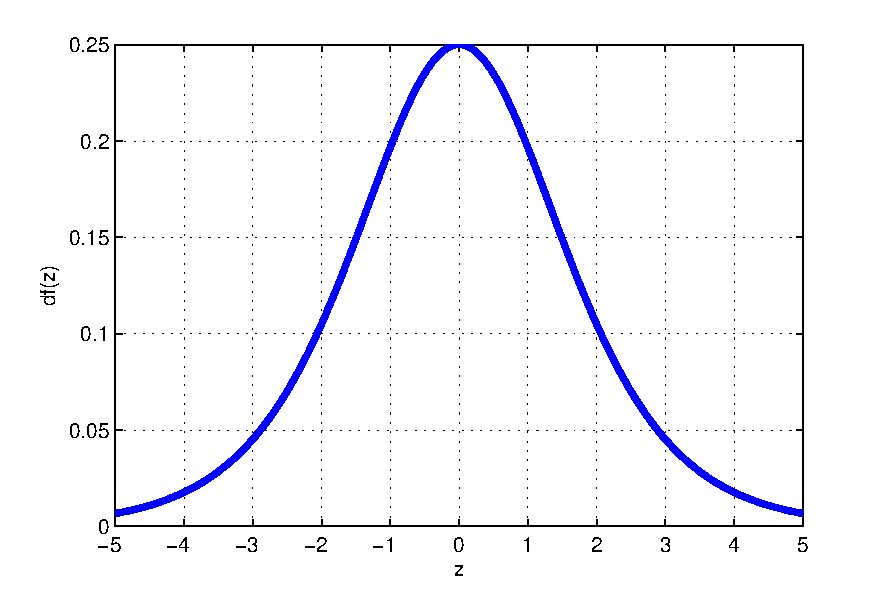
\includegraphics[scale=0.5]{dsigmoid.pdf}
\caption{Plot of first order derivative of Sigmoid function}
\end{center}
\end{figure}


\newproblem{1pt}
We can approximate derivatives numerically
\[
\frac{df(z)}{dz}\approx \frac{f(z+h) - f(z)}{h}
\]
where the right-side of this approximate equality is called {\em finite difference} approximation. Unlike derivative definition we do not need $h$ to be infinitesimal, just a small value. The numerical approximation of a derivative is tremendously useful trick to check you derivative, gradients, Jacobians, Hessians etc. Make sure that you understand what it does.

We will use this approximation to check your derivatives. Here is a function that computes approximately the derivatives of sigmoid
\begin{verbatim}
function d = fdsigmoid(z)
f0 = 1/(1 + exp(-z));
f1 = 1/(1 + exp(-(z + 1e-5)));
d = (f1 - f0)/1e-5;
end
\end{verbatim}
Save this function into a file names \texttt{fdsigmoid.m}.

Try following code in MATLAB
\begin{verbatim}
zs = randn(100,1);
for i=1:length(zs)
    err(i) = dsigmoid(zs(i)) - fdsigmoid(zs(i));
end
hist(err,30)
hwplotprep
print -dpdf hist.pdf
\end{verbatim}
The code above samples 100 normally distributed values and computes the finite differences approximation and the derivative you derived and implemented and then plots histogram of errors.

Find the resulting plot in file {\tt hist.pdf}. In hw\theHW.tex replace {\tt emptiness.pdf} with {\tt hist.pdf} . Change the
caption in the figure to say what the figure is about. Remake hw\theHW.pdf and check that your plot has made it in.
\begin{figure}[H]
\begin{center}
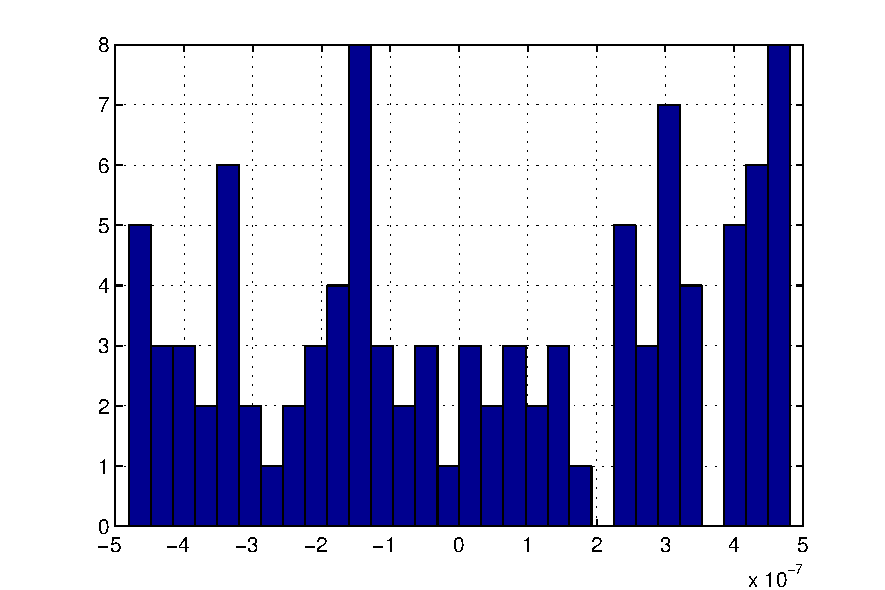
\includegraphics[scale=0.5]{hist_perma.pdf}
\caption{Histogram plot of errors between finite difference approximation and actual first order derivative of Sigmoid function}
\end{center}
\end{figure}


\begin{remark} The error ranges between $-4.7959 \times e^{-07}$ and $4.8082 \times e^{-07}$.
\end{remark}

\newproblem{1pt}
From Taylor's theorem (first year calculus) we can obtain
\[
f(z+h) = f(z) + \frac{df(z)}{dz}h + \frac{1}{2}\frac{d^2f(z)}{d^2z}h^2 + O(h^3).
\]
Derive a bound on the error of the finite differences approximation using the above expression. You can use big O notation to express this bound.
\[
\textrm{Err}(z_0,h) = \abs{\frac{f(z_0+h) - f(z_0)}{h} - \frac{df(z_0)}{dz}} \leq \frac{1}{2} \frac{d^{2}f(z_{0})}{d{z_{0}}^{2}} h + \frac{O(h^{3})}{h}
\]

Specifically for sigmoid function plug in appropriate derivative on the right hand side of the inequality. If $h=10^{-5}$ and $z_0 = 0$ the error of the finite difference should be about $\frac{O(h^{3})}{h} = 10^{-5 \times 2} = 10^{-10}$.

Does this agree with the histogram of error that is in the figure above?

\textbf{Ans.} At $h=10^{-5}$ and $z_0 = 0$ the error of the finite differences and actual derivative (See prob 6 (histogram)) is $9.4645 \times e^{-12}$. As per the above inequality, the difference is $10^{-10}$. They are \textbf{in agreement} ( $9.4645 \times e^{-12} <= 10^{-10}$ ).

\newproblem{1pt}
Let
\BEQ\label{eq:pz}
f(z) = \frac{1}{1 + \myexp{-z}} = p
\EEQ
express $z$ in terms of $p$
\[
z = \ln{(\frac{p}{1-p})}.
\]
Now suppose
\BEQ\label{eq:qz}
\frac{\myexp{-z}}{1 + \myexp{-z}} = q
\EEQ
and express $z$ in terms of $q$
\[
z = \ln{(\frac{1-q}{q})}.
\]
Given Eqs.\eqref{eq:pz},\eqref{eq:qz} express $q$ in terms of $p$
\[
q = 1-p. 
\]
Express $f(-z)$ in terms of $f(z)$
\[
f(-z) = 1 - f(z).
\]
Hint: the manipulations that are useful here are either subtraction from 1 (as in $1-x$), computing inverse (as in $\frac{1}{x}$), and taking logarithm (as in $\log(x)$).

\section*{Log of sigmoid}
\newproblem{1pt}

Let $g(z)$ be log of sigmoid function
\[
g(z) = \mylog{ \frac{1}{1+ \myexp{-z}} }.
\]
Compute its derivative and fill it in here
\[
\frac{dg(z)}{dz} = \frac{1}{\frac{1}{1+e^{-z}}} \frac{d}{dz}(\frac{1}{1+e^{-z}}) = (1+e^{-z}) \frac{1}{e^{z}(1+e^{-z})^{2}} = \frac{1}{e^{z}(1+e^{-z})}.
\]

\[
\frac{dg(z)}{dz} = \frac{1}{1+e^{z}}.
\]

Check your derivative by comparing its value to the finite difference approximation.

\newproblem{1pt}
Compute second derivative of $g(z)$
\[
\frac{d^{2}g(z)}{dz^{2}} = \frac{d}{dz}(\frac{1}{1+e^{z}}) = -1 (1+e^{z})^{-2} e^{z}.
\]
\[
\frac{d^{2}g(z)}{dz^{2}} = \frac{-e^{z}}{(1+e^{z})^{2}}.
\]
Check the second derivative by comparing its value to the finite difference of the {\em first} derivatives you computed above.


\newproblem{1pt}
Let the dataset be specified by $\mathcal{D} = \left\{ (\xx_i,y_i):i=1,\dots,n \right\}$. We specify conditional probability of $y$
\BEQ \label{eq:plr}
p(y | \xx_i,\beta_0,\beta) = \frac{1}{1 + \myexp{-y_i(\beta_0 + \bket{\beta}{\xx_i})}}
\EEQ
Write a matlab function that computes log probability of label $y$ given a vector of features $\xx$ and $\beta_0,\beta$.
\begin{verbatim}
function logP = logProbLogReg(y,X,beta0,beta)
    logP = log(1 ./ (1 + exp(-1 .* y .* (beta0 + X * beta))));
end
\end{verbatim}

Now write a matlab function that uses the above function to compute log probability of label $+1$ for a vector of features $\xx$ and $\beta_0,\beta$
\begin{verbatim}
function predY = predictY(X, beta0, beta)
    logProbY = logProbLogReg(1, X, beta0, beta);
    if logProbY > log(0.5)
        predY = +1;
    else
        predY = -1;
    end
end
\end{verbatim}

\newproblem{1pt}
Given Eq.\eqref{eq:plr} we can write out log-likelihood
\BEQ \label{eq:ll}
\textrm{LL}(\beta_0,\beta;\mathcal{D}) = \sum_i \log \frac{1}{1 + \myexp{-y_i(\beta_0 + \bket{\beta}{\xx_i})}}.
\EEQ
Now using function $\texttt{logProbLogReg}$ that you obtained for the previous problem, write a matlab function that computes loglikelihood
\begin{verbatim}
function val = LogLikLogReg(y,X,beta0,beta)
    val = 0;
    for i=1:length(y)
        val = val + logProbLogReg(y(i), X(i,:), beta0, beta);
    end
end
\end{verbatim}
\newproblem{1pt}
Write a function that computes gradient of log-likelihood of logistic regression Eq.\eqref{eq:ll}
\begin{verbatim}
function [dbeta0,dbeta] = dLogLikLogReg(y,X,beta0,beta)
    dbeta0 = sum(y ./ (1 + exp(y .* (beta0 + X * beta))));
    for j=1:length(beta)
        dbeta(j) = sum( (y .* X(:,j)) ./ (1 + exp(y .* (beta0 + X * beta))));            
    end
end
\end{verbatim}
You can make sure that your implementation is correct using the finite differences trick.
\newproblem{1pt}
Implement a gradient ascent algorithm for fitting logistic regression and paste it below.
\begin{verbatim}
function [beta0, beta] = fitLogReg(y, X)    
    %initialize beta0 and beta
    beta0 = 0;
    beta = zeros(size(X, 2),1);

    %initialize gradients
    dbeta0 = 1;
    dbeta = zeros(size(X,2), 1);
    
    % initialize step size (or learning rate) and max iterations
    eta = 1e-5; % learning rate or step size    
    it = 0; 
    itmax = 2000; % maximum number of iterations    
        
    while (sum(abs(dbeta)) + abs(dbeta0)) > 1e-10 % continue whilst gradient is large        
        % increment the number of updates carried out
        it = it + 1; 
        
        % reset gradients
        dbeta0 = 0; 
        dbeta = 0 * dbeta;
        
        % compute gradients
        dbeta0 = sum(y ./ (1 + exp(y .* (beta0 + X * beta))));
                
        for j = 1 : length(beta)                            
            dbeta(j) = sum( (y .* X(:,j)) ./ (1 + exp(y .* (beta0 + X * beta))));
        end
        
        % update beta0 and beta
        beta0 = beta0 + eta .* dbeta0;
        beta = beta + eta .* dbeta;        

        % break out if max iterations has been reached
        if it > itmax
            break; 
        end
    end   
end
\end{verbatim}

Run it with fixed step size $s=1e-5$, for 2000 iterations, on data stored in \texttt{hw\theHW.mat}.
Note that \texttt{load hw\theHW.mat} loads the $y$ and $X$ variables, on which you can run by issuing command
\texttt{[beta0,beta] = fitLogReg(y,X)}.
Report resulting $\beta_0,\beta$
\begin{verbatim}
beta0 = 0.0010957
beta = [-0.02143 0.1607 -0.01822 -0.04918 -0.04604 -0.04639 0.01162
        -0.0135 -0.02906 -0.0188 -0.0289 -0.03046 0.05342 0.03906
        -0.002518 -0.02692 -0.04047 -0.01994 -0.004227 0.0609 0.008589
        -0.06795 -0.00126 0.03886 0.05141 -0.0403 0.008485 0.1646
        0.1339 -0.02296 -0.003384 0.1003 0.006759 0.124 0.04619
        -0.04314 -0.009258 -0.02412 0.00347 -0.00027 0.01741 0.01438
        -0.003812 -0.01127 -0.02109 -0.008545 0.01536 -0.04617 0.08574
        -0.001652 0.003295 -0.001149 0.01731 -0.01149 0.00503 0.02695
        -0.01551 0.004767 -0.001546 0.00791 0.0126 0.00849 -0.01074
        -0.00753 0.01142 -0.0002641 -0.0001921 -0.00126 -0.006484 -0.0002133
        -0.01787 -0.005508 -0.01482 -7.031e-005 0.003101 0.001028 -0.03209
        0.001426 -0.04631 0.001077 0.01083 0.002858 -0.05803 -0.01238
        -0.02531 -0.0473 0.0009134 -0.001276 -0.2578 -0.03866 -0.05325
        0.001799 0.01528 0.01037 -0.0326 0.01012 -0.007789 -0.006569
        -0.01981 -0.001454 0.0006085 -0.01635 -0.000497 -0.0006021 -0.02542
        0.0001593 -0.09198 0.1555 0.01523 -0.08047 0.06645 0.009665
        -0.1879 0.07071 -0.2866 0.1835 0.04374 0.0006091 -0.05094
        0.08198 0.01465 0.06707 0.01884 0.1883 0.009685 0.0434
        0.00253 0.02507 -0.01647 0.003903 -0.03436 -0.02429 0.03313
        0.003609 0.00776 0.02836 0.05266 0.009622 0.02063 0.0359
        0.03319 0.02649 0.01353 0.05517 0.02412 0.0346 0.03049
        0.03749 0.04143 0.004976 -0.01309 -0.01127 0.02519 -0.02121
        0.01663 -0.02574 -0.0211 -0.04929 -0.03417 -0.01576 -0.03091
        -0.02881 -0.03066 -0.04566 -0.04843 0.0002199 -0.05544 -0.01424
        -0.004019 -0.01473 -0.03598 -0.02181 0.002669 -0.03686 -0.0008104
        -0.0184 -0.006603 -0.02072 -0.02646 -0.002791 0.04217 0.04199
        0.003642 0.03562 0.03278 0.04564 0.008575 0.01454 -0.01995
        0.04076 0.01194 0.02964 0.03056 0.00102 -0.01413 0.008393
        0.02805 0.02004 0.01452 0.01527 0.04959 0.03062 0.04593
        0.002911 -0.00366 -0.02184 -0.01791 -0.0217 0.02037 -0.03698
        0.006691 -0.005006 0.009788 0.00524 0.002131 0.02802 0.02835
        -0.009176 0.004066 -0.02371 -0.03402 -0.03748 0.009218 -0.004869
        -0.02866 -0.03108 0.0121 -0.03262 -0.01632 -0.04654 0.007686
        -0.0789 0.007168 -0.01708 0.01133 -0.02453
       ]
\end{verbatim}
\newproblem{1pt}
Implement estimation of prediction error using cross validation
\begin{verbatim}
load  hw1.mat
X = X';
y = y';
rand('seed',1);
K  =  5;
N  =  length(y);
indices  =  crossvalind('Kfold',N,K);
err = zeros(K, 1);
err1 = zeros(K, 1);

for  k = 1 : K
    testX  =  X(indices  ==  k,:);
    testY  =  y(indices  ==  k);    
    trainX  =  X(indices  ~=  k,:);
    trainY  =  y(indices  ~=  k);    
    [beta0,beta]  =  fitLogReg(trainY, trainX);    
    
    predY = zeros(1, size(testY, 1));
    for  i=1:length(testY)
        predY(i) = beta0 + testX(i,:) * beta;        
        err(k) = err(k) + abs(testY(i)-predY(i));
    end   
end

cvErr  =  sum(err)/length(y);
display(cvErr);
\end{verbatim}
Once done, run this on data stored in \texttt{hw\theHW.mat}. The cross-validation estimate of error on that dataset is $1.1363$.
\end{document}
